El problema que se nos presenta es, dados $k$ vectores ordenados de menor a mayor,
cada uno con $n$ elementos, combinarlos en un único vector con todos los elementos
ordenados de la misma manera. Al igual que antes, presentamos una solución obvia y
otra empleando un algoritmo Divide y Vencerás. 

\subsection{Caso obvio}

En este caso una alternativa es ir iterando sobre cada vector, añadiendo los elementos
del vector de forma ordenada sobre un acumulador. Ello queda ilustrado en la figura
\ref{fig:2a-obvio}, donde primer se unen los vectores que están en rojo y morado para,
a continuación, unir ese resultado con el vector en verde, dando como resultado
un vector global ordenado. 

\begin{figure}
    \centering
    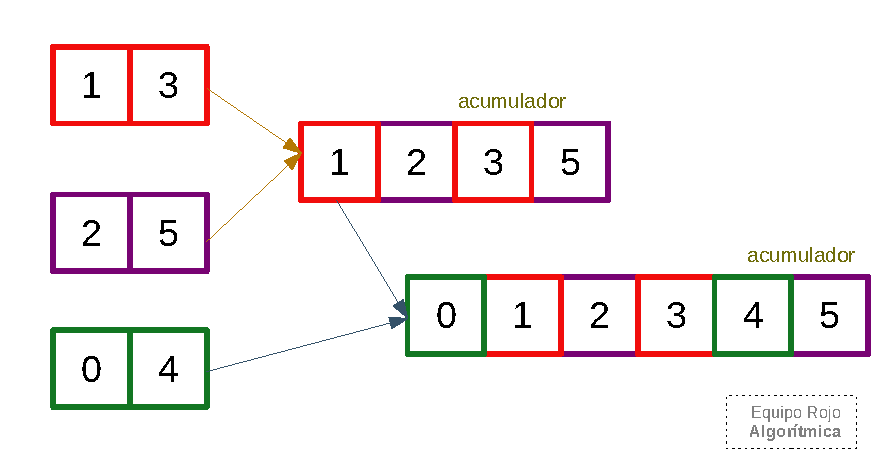
\includegraphics[scale=0.87]{img/orden_2a.pdf}
    \caption{Esquema de funcionamiento del algoritmo de 
    mezcla obvio. Elaboración propia.}
    \label{fig:2a-obvio}
\end{figure}

\subsubsection{Pseudocódigo}

